% Chapter X

\chapter{Infection of \textit{Acanthamoeba castellanii} by \textit{Legionella pneumophila}} % Chapter title

\label{ch:02-02} % For referencing the chapter elsewhere, use \autoref{ch:name} 

%----------------------------------------------------------------------------------------

Legionella pneumophila alters its host signal transduction, metabolism and gene regulation upon infection. In addition to all these changes, it also affects host histone marks, which are known to be related to gene regulation and genome architecture. In this chapter, we investigate the genome structure of \textit{A. castellanii} and how it is affected during infection by \textit{L. pneumophila}.

\section{Genome assembly}

As with most other genomics techniques, a prerequisite of Hi-C analyses is to have a high quality reference genome with clearly delimited chromosomes. At the time of writing, the A. castellanii reference genome is split into 384 scaffolds which do not represent chromosomes. This prompted us to generate a chromosome-level genome assembly.

\section{Genome architecture of \textit{A. castellanii}}

The genome of \textit{A. castellanii} is 45Mbp long and pulsed field gel electrophoresis experiments suggested that it has around 20 chromosomes \cite{rimmResolutionAcanthamoebaCastellanii1988}. The 5S ribosomal DNAs are dispered throughout all chromosomes, unlike in most species, where they are clustered in tandem repeats.

\section{Strains comparison}

Several strains of \textit{A. castellanii} have been isolated throughout history.These strains may originate from different ecological niche of geographical location and have been cultivated in labs for long preriods. As a result, they can differ in various phenotypes, including susceptibility to infection. Comparing such divergent strains can help us understand what genomic features are important for pathogen susceptibility.


\section{Changes during infection}

\begin{figure}[b]
    \includegraphics[width=\textwidth]{Parts/Part02/gfx/acastellanii_interchrom.pdf}
    \caption[Interchromosomal contacts changes during infection by \textit{Legionella}.]{Interchromosomal contacts changes during infection by \textit{Legionella}: \textbf{a:} Whole genome contact map of \textit{A. castellanii str. C3} and log ratio map of \textit{L. pneumophila}-infected over control. Green lines delimit scaffolds. \textbf{b:} Mean contact changes during infection between all pairs of chromosomes before (left) and after(right) clustering chromosomes.}
	\label{fig:02-02:inter-infection}
\end{figure}


\begin{figure}[b]
    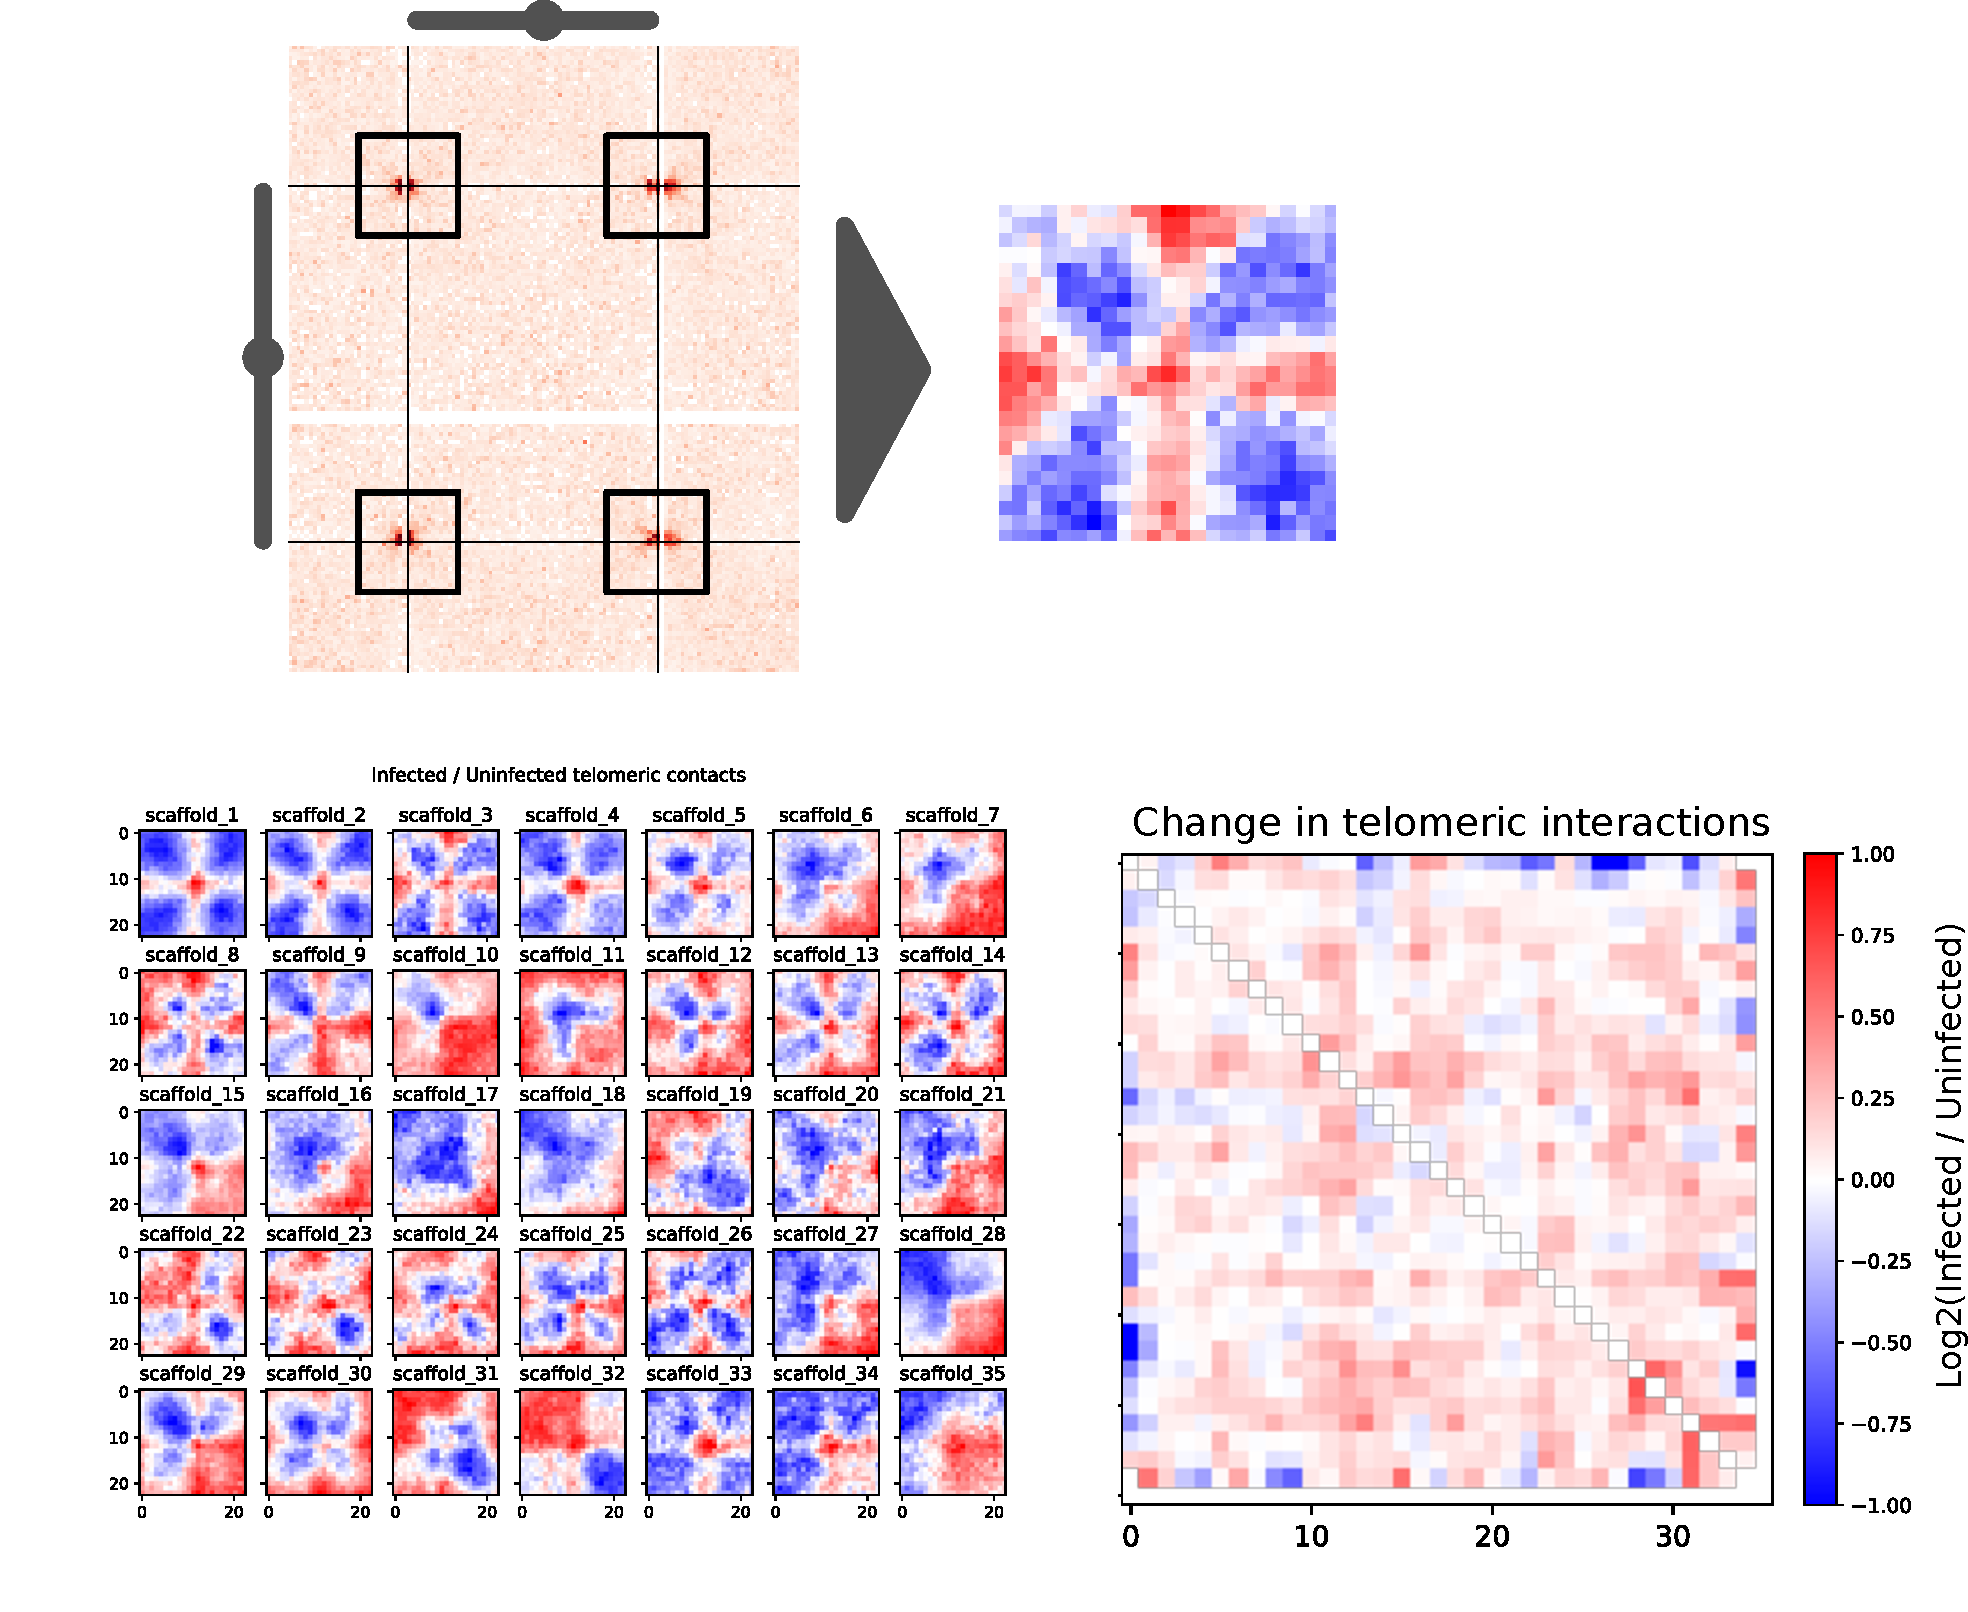
\includegraphics[width=\textwidth]{Parts/Part02/gfx/acastellanii_telomeres.pdf}
    \caption[Telomeric interactions changes during infection by \textit{Legionella}.]{Telomeric interactions changes during infection by \textit{Legionella}: \textbf{a:} Illustration of the extraction process for inter-telomeric contact from two chromosomes. All telomeric windows are  into a pileup for a given chromosome and the ratio between infected (I) and uninfected (U) pileups can be visualised. Change in telomeric pattern intensity during infection for all pairs of chromosomes. The intensity is the Pearson correlation coefficient between the telomeric pileup and each telomeric window. Each value in the matrix represents a pair of chromosome, consisting of the average of 4 telomeric windows. Intrachromosomal windows are excluded. \textbf{b:} Telomeric contacts ratio for all chromosomes. For each chromosome, the pileup contains the windows of its telomeric interactions with all other chromosomes.}
	\label{fig:02-02:telo-infection}
\end{figure}